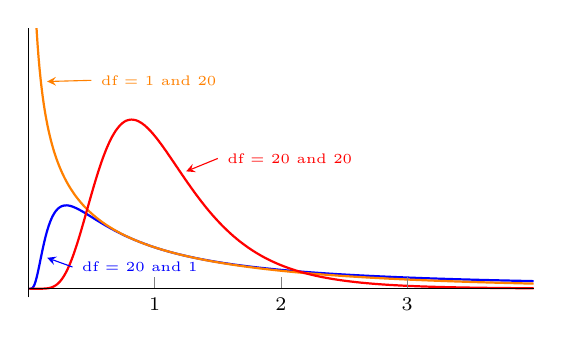
\begin{tikzpicture}[
    declare function={
        gamma(\z)=2.506628274631*sqrt(1/\z)+ 0.20888568*(1/\z)^(1.5)+ 0.00870357*(1/\z)^(2.5)- (174.2106599*(1/\z)^(3.5))/25920- (715.6423511*(1/\z)^(4.5))/1244160)*exp((-ln(1/\z)-1)*\z;
    },
    declare function={
        beta(\x,\y)=gamma(\x)*gamma(\y)/gamma(\x+\y);
    },
    declare function={
        fdist(\x,\a,\b) = 1 / beta(\a/2, \b/2) * (\a/\b)^(\a/2) * \x^(\a/2-1) * (1 + \a/\b*\x)^(-(\a + \b)/2);
    }
  ]
    \begin{axis}[
        axis lines*=middle,
        no markers,
        domain=0.01:4,
        samples=500,
        xmin = 0, xmax = 4,
        ymin = -0.05, ymax = 1.5,
        xtick={0,1,2,3},
        ticklabel style={font=\scriptsize},
        ytick=\empty,
        grid = none,
        axis on top,
        height=5cm,
        width=8cm
      ]
      \addplot+[thick,blue] { fdist(x, 20,1) };
      \addplot+[thick,orange] { fdist(x, 1,20) };
      \addplot+[thick,red] { fdist(x, 20,20) };
      \node[blue,right] (A) at (0.35,0.125) {\tiny df = 20 and 1};
      \node[orange,right] (B) at (0.5,1.2) {\tiny df = 1 and 20};
      \node[red,right] (C) at (1.5,0.75) {\tiny df = 20 and 20};
      \draw[blue,-stealth] (A.180) -- (axis cs: 0.15, {fdist(0.1,20,1)});
      \draw[orange,-stealth] (B.180) -- (axis cs: 0.15, {fdist(0.1,1,20)});
      \draw[red,-stealth] (C.180) -- (axis cs: 1.25, {fdist(1.2,20,20)});
    \end{axis}
\end{tikzpicture}